\documentclass[a4paper, 12pt, oneside, titlepage, openany]{book}

\usepackage{titlesec} %Para el seccionado, debe colocarse al principio este package.

%Interlineado de todo el documento a 1.5
\usepackage{setspace}
%\spacing{1.5} ir\'a en diferentes secciones

\usepackage{color,soulutf8}
\usepackage{float}
\floatstyle{boxed}
\restylefloat{table}
\restylefloat{figure}
\usepackage[section,above,below]{placeins}
\usepackage{microtype}
\usepackage{amsmath,amsfonts,amssymb}
\allowdisplaybreaks
\usepackage{stmaryrd}
\SetSymbolFont{stmry}{bold}{U}{stmry}{m}{n}
\usepackage[braket]{qcircuit}
\usepackage{proof}
\usepackage{tikz}
\usepackage{multicol,multirow}
\usepackage{graphicx}
\usepackage{array,longtable}
\usepackage{wrapfig}
\usepackage{commath}
\usepackage{MnSymbol}
\usepackage{anyfontsize}% permite tamaño de fuentes arbitrarios
\usepackage{tikz, pgfplots}
\pgfplotsset{compat=newest}
\usepackage{hyperref}

% automatic math mode, centered
\newcolumntype{C}{>{$}c<{$}}
\newcolumntype{R}{>{$}r<{$}}
\newcolumntype{L}{>{$}l<{$}}

\newtheorem{theorem}{Teorema}[section]
\newtheorem{lemma}[theorem]{Lema}
\newtheorem{corollary}[theorem]{Colorario}
\newtheorem{proposition}[theorem]{Proposicion}

\newenvironment{definition}[1][Definici\'on]{\begin{trivlist}
%Como en el libro de Tromba, an\'alisis Matem\'atico. En negrita y sin enumeraci\'on:
\item[\hskip \labelsep {\bfseries #1}]}{\end{trivlist}} 
\newenvironment{exercise}[1][Ejercicio]{\begin{trivlist}
\item[\hskip \labelsep {\bfseries #1}]}{\end{trivlist}} 
\newenvironment{proof}[1][Demostraci\'on]{\begin{trivlist}
\item[\hskip \labelsep {\itshape #1}]}{\end{trivlist}}
\newenvironment{example}[1][Ejemplo]{\begin{trivlist}
\item[\hskip \labelsep {\itshape #1}]}{\end{trivlist}}
\newenvironment{remark}[1][Comentario]{\begin{trivlist}
\item[\hskip \labelsep {\itshape #1}]}{\end{trivlist}}

\usepackage{lastpage}
\usepackage{titleps}

\newpagestyle{ruled}
%En los tres corchetes, para izq, centro, der, paginas pares. En llaves, paginas impares.
%Solo llaves es para ambas paginas.
	{   
   %\sethead{
\includegraphics[width=3.7cm]{./images/UADE_LARGE}}{\Title}{\Author}\headrule
	\sethead{
\includegraphics[width=3.7cm]{./images/UADE_LARGE}}
			{\parbox[b]{0.43\textwidth}{\centering AN\'ALISIS MATEM\'ATICO 3}} %b es para poner texto sobre el bottom
			{Nicolás Alberto Monzón}\headrule
	\setfoot[][][P\'agina \thepage\ de \pageref{LastPage}]{}{}{P\'agina \thepage\ de \pageref{LastPage}}\footrule
	}
	\pagestyle{ruled}
%Cambiar el color de la linea divisora:
%\renewcommand\makeheadrule{\color{cyan}\rule[-.3\baselineskip]{\linewidth}{0.4pt}}
%\renewcommand\makefootrule{\color{cyan}\rule[\baselineskip]{\linewidth}{0.4pt}}

%M\'argenes
\usepackage{vmargin}
%\setmarginsrb{leftmargin}{topmargin}{rightmargin}{bottommargin}%
%         {headheight}{headsep}{footheight}{footskip}           %
%Lo ideal ser\'ia lo siguiente
%\setmarginsrb{2.7cm}{4cm}{2.3cm}{2.5cm}{2cm}{0.5cm}{2cm}{0.5cm}
%Pero estos valores se suman, por lo que en realidad ir\'ia asi:
\setmarginsrb{2.7cm}{2cm}{2.3cm}{1.5cm}{0cm}{2cm}{0cm}{1cm}

%M\'argenes, pero otra opci\'on mas acotada
%\usepackage[top=4cm,bottom=2.5cm,left=2.7cm,right=2.3cm]{geometry}

%Se decidi\'0 no usar Babel, para no romper con otros paquetes sólo para unas pocas traducciones
%Nombre de cap\'itulos
\renewcommand{\chaptername}{Cap\'itulo} %Falta verificar si es correcto que esto se vea.
\renewcommand{\bibname}{Bibliograf\'ia}
\renewcommand{\contentsname}{\'Indice}
\renewcommand{\listfigurename}{Lista de Figuras}
\renewcommand{\listtablename}{Lista de Tablas}
\renewcommand{\appendixname}{Ap\'endice}
%\renewcommand\appendixpagename{Ap\'endice}
\renewcommand\tablename{Tabla}
\renewcommand{\figurename}{Figura}

%Para que el primer parrafo de un cap\'itulo tenga identado.
\usepackage{indentfirst}
\setlength{\parindent}{12pt} %Tamaño de la identaci\'on.

%Seccionado. El par\'ametro left incrementa el margen, lo setteo en 0.
%\titlespacing*{<command>}{<left>}{<before-sep>}{<after-sep>}
\titlespacing{\section}{0pt}{20pt}{20pt}
%\titlespacing{\subsection}{0pt}{*0}{*0}
%\titlespacing{\subsubsection}{0pt}{*0}{*0}

%Tamaño de letra de cap\'itulo y secciones
\newcommand{\chapfnt}{\fontsize{16}{19}}
\newcommand{\secfnt}{\fontsize{14}{17}}
%\newcommand{\ssecfnt}{\fontsize{12}{14}}
\titleformat{\chapter}[display]
{\normalfont\chapfnt\bfseries}{\chaptertitlename\ \thechapter}{20pt}{\chapfnt}
\titleformat{\section}
{\normalfont\secfnt\bfseries}{\thesection}{1em}{}
%\titleformat{\subsection}
%{\normalfont\ssecfnt\bfseries}{\thesubsection}{1em}{}

%Se pide numeraci\'on de tablas en n\'umeros romanos
\renewcommand{\thetable}{\Roman{table}}

%Espaciado antes y despu\'es de una figura respecto del texto
\setlength{\textfloatsep}{5pt}

%Espaciado entre referencias en la bibliograf\'ia
\usepackage{etoolbox}
\patchcmd{\thebibliography}
  {\settowidth}
  {\setlength{\itemsep}{6pt}\settowidth}
  {}{}
\apptocmd{\thebibliography}
  {\small}
  {}{}
  
\usepgfplotslibrary{patchplots}

\pgfplotsset{compat=1.10}
\usepgfplotslibrary{fillbetween}
\usetikzlibrary{patterns}

\begin{document}

%\maketitle

\begin{titlepage}

	\centering
	%\fontsize{<size>}{<bskip>}
	{\textbf{\fontsize{16}{17}\selectfont AN\'ALISIS MATEM\'ATICO 3} \par}
	\vspace{1cm}
	{\textbf{\fontsize{16}{17}\selectfont Monz\'on, Nicol\'as Alberto - LU 1070224} \par}
	\vspace{1.5cm}
	{\fontsize{16}{17}\selectfont Ingenier\'ia en Inform\'atica \par}
	\vspace{1cm}
	{\textbf{\fontsize{14}{14}\selectfont Profesor:} \par}
	{\fontsize{14}{14}\selectfont Avila, Silvia Beatriz (siavila@uade.edu.ar)
	\par}
	\vspace{1cm}
	{\textbf{\fontsize{14}{14}\selectfont Ayudante de 1ra:} \par}
	{\fontsize{14}{14}\selectfont Schifani, Guido (gschifani@uade.edu.ar)
	\par}
	\vfill
		v1.0.0
	\vfill
	
\includegraphics[width=0.30\textwidth]{./images/UADE}\par \vspace{1cm}
	{\textbf{\fontsize{14}{14}\selectfont UNIVERSIDAD ARGENTINA DE LA EMPRESA} \par}
	{\fontsize{14}{14}\selectfont FACULTAD DE INGENIER\'IA Y CIENCIAS EXACTAS \par}

\end{titlepage}

\chapter*{Notas Preliminares}
Los trabajos pr\'acticos son los dados en la materia, no hay ning\'un ejercicio propio propuesto dentro de los resueltos.

\tableofcontents

\chapter{Integrales curvil\'ineas}
\section{Integral doble sobre rect\'angulos}

Sea $f: \mathcal{D} \subseteq \mathbb{R}^2 \rightarrow \mathbb{R}$, $z = f(x,y)$ y sea $\mathcal{R} \subset \mathcal{D}$ un rect\'angulo, se lo puede definir como
$$
\mathcal{R} = \left[a,b\right] \times \left[c,d\right] = \lbrace (x,y) \in \mathbb{R}^2: a \leq x \leq b, c \leq y \leq d \rbrace
$$
Teniendo $f(x,y) \geq 0 \forall(x,y) \in \mathcal{R}$. Sea el macizo $M = \lbrace (x,y,z) \in \mathbb{R}^3: (x,y) \in \mathcal{R},0 \leq z\leq f(x,y)$



\section{Ejercicios}

\begin{enumerate}

\item Calcular, siempre que exista, la integral doble $I(f,\mathcal{R}) = \iint_{\mathcal{R}}f(x,y)dxdy$ en el recinto $\mathcal{R} \subset \mathcal{D} \subset \mathbb{R}^2$ del campo escalar $f: \mathcal{D} \rightarrow \mathbb{R}$. Graficar el recinto $\mathcal{R}$ en el que se integra y calcular su \'area $A(\mathcal{R})$. Determinar, adem\'as, el valor medio $$\mu(f,\mathcal{R}) = \frac{\iint_{\mathcal{R}}f(x,y)dxdy}{\iint_{\mathcal{R}}dxdy}$$ del campo escalar en el recinto\footnote{Si, por ejemplo, la funci\'on $f$ representa una densidad superficial, el valor medio en la l\'amina $\mathcal{R}$ es la densidad media. Una l\'amina $\mathcal{R}$ homog\'enea de densidad igual a la densidad media, tiene la misma masa que la l\'amina original de densidad variable dada por la funci\'on $f$}.
\begin{enumerate}
	\item $\mathcal{R} = \left[ 0, 1 \right] \times \left[ 0, 2 \right], f: \mathbb{R}^2 \rightarrow \mathbb{R} \textrm{ tal que } f(x,y) = 3x^2 + 2y$.
\end{enumerate}

\end{enumerate}

\section{Claves de correcci\'on}

\begin{exercise}

(1a)\\
Respuesta a realizar.
%h (here), le decimos que ponga la imagen m\'as o menos aqu\'i
%t (top), preferiblemente en la parte superior de la p\'agina
%b (bottom), preferiblemente en la parte inferior de la p\'agina
%p (page), que junte los objetos flotantes en una p\'agina
%! que ignore sus reglas internas de posicionamiento
%H que ponga la imagen justo aqu\'i, similar a h!
\begin{figure}[h]
\centering
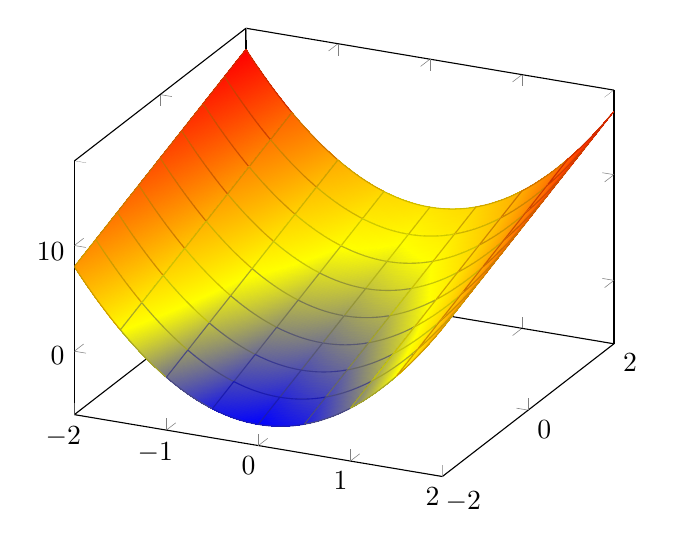
\begin{tikzpicture}
    \begin{axis}
    \addplot3[patch,patch refines=3,
		shader=faceted interp,
		patch type=biquadratic] 
    table[z expr=3*x^2 + 2*y]
    {
        x  y
        -2 -2
        2  -2
        2  2
        -2 2
        0  -2
        2  0
        0  2
        -2 0
        0  0
    };
    \end{axis}
\end{tikzpicture}
\caption{Gr\'afico de $f(x,y) = 3x^2 + 2y$}
\label{fig:exercice_01_a_01}
\end{figure}

\end{exercise}

\chapter{Integrales m\'ultiples}
A completar
 
\chapter{Integrales de superficie}
A completar

\chapter{Ecuaciones diferenciales de primer orden}
\section{Funci\'on escal\'on (Heaviside)}

Usamos la notaci\'on $u$ por "unitario", por ser "un" escal\'on, o $h$ por \emph{Heavside}.

%Acá va la gráfica de Heaviside, y una muestra de como queda simplificada (con la línea pintada en lugar de punteada, como si no fuera una función).

$$
u(t) = \lbrace{ \begin{matrix}
0 \textrm{ si } t \leq 0 \\
1 \textrm{ si } t > 0
\end{matrix} }
$$

%Colocar los gráficos de ejemplo de las siguientes funciones:

$$f(t) = t^2u(t)$$
$$g(t) = t^2u(t+1)$$
$$h(t) = t^2u(1-t)$$
$$z(t) = t^2(u(t) - u(t-1))$$ %Es un peldaño
%Graficar la formula general u(t-a) - u(t- b) que es una onda cuadrada, que solo grafica de a hasta b.
$$w(t) = (t-1)^2 u(t-1)$$ 

\begin{definition}
(Transformada de Laplace) Sea $f: \mathcal{D}_f \subset \mathbb{R} \rightarrow \mathbb{R}$, se llama Transformada de Laplace (TL) de la funci\'on $f$ y se escribe $\mathcal{L}(f)(p) = \int_{0}^{\infty}e^{-pt}f(t)dt$ (si existe).
\end{definition}

Esto lo que nos dice que es que tenemos una funci\'on $f$, con una variable (por ejemplo $t$), que al ser evaluada por $\mathcal{L}$ tenemos una nueva funci\'on (llamada $F$) que tiene una nueva variable $p$.

%Colocar un ejemplo de una función, con una flecha que muestre que tiende  aun nuevo grafico de F.

Si la integral existe, entonces $f$ es $\mathcal{L}$-transformable (en caso contrario no tiene TL).
\emph{Observaci\'on}: la "cola izquierda" (si la tiene) de $f$ no se tiene en cuenta, as\'i que tenemos
$$
\int_{0}^{\infty}e^{-pt}f(t)u(t)dt
$$

Veamos un ejemplo de TL.

%Poner encima del singo igual "def"
$$
U(p) = \int_0^{\infty}e^{-pt}u(t)dt
$$
Como $u(t)$ vale 1 donde estoy integrando,
$$
= \int_0^{\infty}e^{-pt}dt = (-\frac{1}{p}e^{-pt})\|^{\infty}_0
$$
Como $p > 0$
$$
= (-\frac{1}{p}\left[0 - 1\right] = \frac{1}{p})
$$

Tenemos que pensar a $p$ como una constante que va a seguir viva luego de la integraci\'on y a $t$ como nuestra variable. La TL de $U(t)$ se define para $p>0$, y esto va a aparecer en la tabla de Laplace.

\emph{Observaci\'on} Una condici\'on suficiente para que existe la TL, es que la funci\'on $f$ sea continua por partes (CPP), y de orden $\alpha$-exponencial\footnote{Esto significa que si tiene discontinuidades, los saltos son finitos (no hay un salto infinito) y que se la puede acotar a partir de un cierto $t$ por una exponencial del tipo $e^{\alpha t}$, en tal caso, por lo menos se puede asegurar que la TL existe para $p > \alpha$}.

%%Hacer grafico explicativo con una función f(t) con una exponencial por encima y poner lo siguiente
$\|f(t)\| \leq M e^{\alpha t}$ ($M$ es un valor constante) %Verificar $\|f(t)\| \leq M e^{\alpha t}$%

%%Hacer otro grafico que muestre que para la exponencial anterior, F(p) tiene una absisa de convergencia, es decir una linea vertical en \alpha que muestra que se grafica desde allí hacia la derecha.

%%Colocar apéndice con tablas de Laplace

Propiedades:

\begin{enumerate}

\item (Verificaci\'on de la transformada) Suponiendo que $f(t)u(t) \longrightarrow F(p)$ %colocar encima de la flecha TL
$tf(t)u(t) \longrightarrow ?$ %colocar encima de la flecha TL, signo de pregunta en rojo
Veamos:
$$
F(p)= \int_0^{\infty}e^{-pt}f(t)dt
$$
Derivamos esta funci\'on (en funci\'on de $p$)
$$
\frac{d}{dp}F(p) = \frac{d}{dp}\int_0^{\infty}e^{-pt}f(t)dt = \int_0^{\infty}\frac{d}{dp}(e^{-pt}f(t))dt
$$
Es decir, pensamos que nuestra integral es transparente a nuestra derivaci\'on, lo cual se debe a propiedades de continuidad que no se van a tocar. Suponemos que esto es verdad por el momento,
$$
= \int_0^{\infty}\frac{d}{dp}((-t) e^{-pt}f(t))dt = -F^{\prime}(p)
$$
Entonces $tf(t)u(t) \longrightarrow -F^{\prime}(p)$. %colocar encima de la flecha TL
Tambi\'en se tiene, en general %%Poner todo esto en una tabla como en mi tesis
$t^n f(t)u(t) \longrightarrow (-1)^n F^{(n)}(p)$.
Por ejemplo: $tu(t) \longrightarrow -(\frac{1}{p}^{\prime}) = -(-\frac{1}{p^2}) = p^{-2}$.

\item $f(t)u(t) \longrightarrow F(p)$, entonces $f^{\prime}(t) = ?$
$$
\mathcal{L}(f^{\prime}(p) = \int_0^{\infty}e^{-pt}f^{\prime}(t)dt
$$%Colocar "def" encima de la flecha
Integro por partes con $u = e^{-pt}$, $du = -p e^{-pt}dt$, $dv = f^{\prime}(t)dt$, $v = f(t)$
$$
=f(t)e^{-pt}\|^{\infty}_0 + \int_0^{\infty}pe^{-pt}f(t)dt = pF(p) - f(0)
$$
Entonces $f^{\prime}(t) = pF(p) - f(0)$. De ac\'a, se tiene que $f^{\prime\prime}(t) \longrightarrow p^2F(p)-pf(0)-f^{\prime}(0)$ %colocar encima de la flecha un TL
Es decir, multiplicamos por $p$ lo que ya teniamos y le restamos lo que acabamos de derivar, en $0$. Para $f^{\prime\prime\prime}(t) \longrightarrow p^3F(p)-p^2f(0) - pf^{\prime}(0) -f^{\prime\prime}(0)$.

\item $f(t)u(t) \longrightarrow F(p)$, entonces $e^{at}f(t)u(t) \longrightarrow ?$ %Colocar TL encima de la flecha.
Calculamos:
$$
\mathcal{L}(e^{at}f(t)u(t))(p) =\int_0^{\infty}e^{-pt}e^{at}f(t)dt = \int_0^{\infty}e^{-(p-a)t}f(t)dt = F(p-a)
$$
$u(t)$ vale $1$ en el \'area de integraci\'on. Entonces $e^{at}f(t)u(t) \longrightarrow F(p-a)$.

Con la propiedad anterior, podemos por definici\'on de $\cosh$ y $\sinh$:
$$
\cosh{at} = \frac{1}{2}(e^{at} + e^{-at}) \longrightarrow \frac{1}{2}(\frac{1}{p-a} + \frac{1}{p+a}) = \frac{p}{p^2-a^2},p>\|a\|
$$ (esto \'ultima dado que por la primera fracci\'on, $p > a$ y por la segunda $p > -a$). %Colocar TL encima de la flecha
$$
\sinh{at} = \frac{1}{2}(e^{at} - e^{-at}) \longrightarrow \frac{1}{2}(\frac{1}{p-a} - \frac{1}{p+a}) = \frac{a}{p^2-a^2},p>\|a\|
$$ (esto \'ultima dado que por la primera fracci\'on, $p > a$ y por la segunda $p > -a$). %Colocar TL encima de la flecha

Podemos combinar propiedades:

$$
t e^{at} u(t) \longrightarrow -\frac{1}{p-a} = \frac{1}{(p-a)^2}
$$ %Colocar TL encima de la flecha

\end{enumerate}

\section{Ejercicios}

\begin{enumerate}

\item Ejercicio 1
\item Ejercicio 2
\item Ejercicio 3 ...

\end{enumerate}

\section{Claves de correcci\'on}

\begin{exercise}
(2a)
$$x = e^{t+1}$$
$$x^{\prime} = e ^{t + 1} = x$$
$$x = x^{\prime}$$
Entonces: $x^{\prime} - x = 0$ EDO.

\end{exercise}

\begin{exercise}
(2c)
$$x = A \sin{t}$$
$$x^{\prime} = A \cos{t}$$
$$x^{\prime \prime} = - A \sin{t}$$
Entonces: $x + x = x^{\prime \prime} = 0$.

\end{exercise}

\begin{exercise}
(3e)

Como nos piden verificar, solo derivamos y reemplazamos. Con $y = y(x)$ en la EDO $1^3 + x = x + 1 = y$, por lo tanto, cumple.
$y = x + 1$ es soluci\'on particular (no hay par\'ametros libres).

\end{exercise}

\begin{exercise}
(4) Incompleto.

Consideramos $y^{\prime} = \frac{dy}{dx}$

\end{exercise}

\begin{exercise}
(7h) Considerando $y^{\prime} + p(x)y = q(x)$
$$y \longrightarrow 1$$
$$x \longrightarrow \infty$$
Tenemos
$$x^{2}y^{\prime} + xy^{\prime} = y - 1$$
$$(x^2 + x)y^{\prime} - y = -1$$
$$y^{\prime} - \frac{1}{x^2 + x}y = - \frac{1}{x^2 + x}$$
Tomamos las funciones
$$g(x) = - \frac{1}{x^2 + x}$$
$$f(x) = - \frac{1}{x^2 + x}$$
Por \emph{factor integrante},
$$\mu(x) = e ^{\int{- \frac{1}{x^2 + x}dx}}$$

C\'alculo auxiliar.

$$
{\int{- \frac{1}{x^2 + x}dx}} = 
{\int{- \frac{1}{x(x + 1)}dx}} =
{\int{(\frac{A}{x} + \frac{B}{x+1})dx}} =
{\int{(\frac{A(x+1) + BX}{x(x+1)}})dx}
$$
$$
A(x+1) + Bx = 1 
$$
Uso $x = 0$, entonces $A = 1$. Si $x = -1$, entonces $B = -1$
$$
={\int{(\frac{1}{x} + \frac{1}{x+1})dx}}
=\ln{x}-\ln{x+1}=ln{\frac{x}{x+1}}
$$

Fin del c\'alculo auxiliar.

Entonces
$$
\mu(x)=e^{-\ln{\frac{x}{x+1}}} = \frac{x}{x+1}^{-1} = \frac{x+1}{x} = 1 + \frac{1}{x}
$$
$$
y = \frac{\int{-\frac{x+1}{x} \frac{1}{x^2 + x}}}{\frac{x+1}{x}}
$$

Partiendo de $(x^2 + x)y^{\prime} - y = 1$ entonces $(x^2 + x)\frac{dy}{dx} = y - 1$, entonces $\frac{dy}{y-1} = \frac{dx}{x^2 + x}$ y, entonces, $\ln{\|y-1\|} = \ln{\|\frac{x}{x+1}\|} + C_1$. Darnos cuenta de que son variables separadas nos da una ventaja m\'as grande. Una forma m\'as r\'apida es ver que si $x\longrightarrow \infty$, entonces dado que $y - 1 = k\frac{x}{x+1}$, entonces, si $y = 1 + k\frac{x}{x+1}$ nos queda $y = 1$. Y es f\'acil verificar entonces que $y^{\prime} = 0$ y cumple la condici\'on inicial.


\end{exercise}
 
\chapter{Ecuaciones diferenciales de orden superior}
A completar

\chapter{Ejemplos de examen}
A completar

\appendix
\chapter{Tabla de integrales}
A completar

\bibliography{biblio}
\addcontentsline{toc}{chapter}{Bibliograf\'ia}
%Las opciones de estilo mencionadas en ISO 690-2 son las siguientes.
%abntex2-num.bst
%El resto son incompatibles.
\bibliographystyle{iso690}

\listoffigures
\listoftables

\end{document}